Calcularemos la capacitancia del condensador cooplanar con la forma mostrada en la \ref{fig:capacitor}, cuyas dimensiones reales son  $2046 \mu m$ de alto y  $2430 \mu m$ de largo (las dimensiones detalladas se muestran en []), Donde la región azul tendrá potencial fijo $\phi_0=0V$, la región roja  $\phi_0=3.5V$ y la región blanca tendrá  $\phi_0=1.6V$ esperando que el metodo converja más rápido. 
\begin{figure}[H]
		\centering
		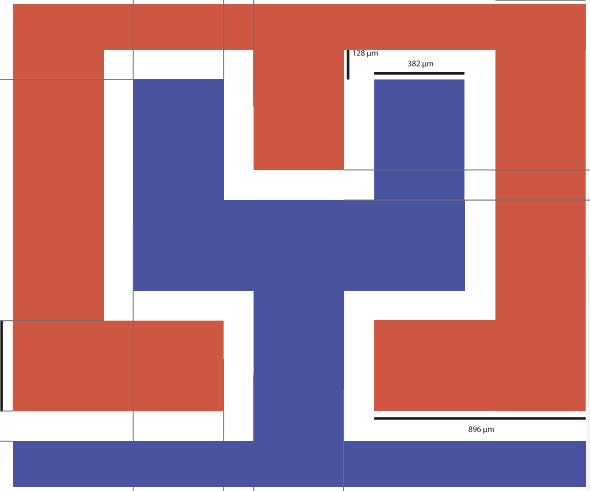
\includegraphics[width=0.8\columnwidth]{img/problema.png}

		\caption{Esquema fotodiodo PN }
		\label{fig:capacitor}
\end{figure}

Se empleo un mallado de $2046 \times 2430$, en un arreglo matricial donde cada entrada de la matriz representa un área de $ 1 \mu m \times  1 \mu m$. 

Se aplico el método \ref{aproxV} en la región blanca, para observar como se comporta el potencial, con este potencial se calcula el campo eléctrico en toda el área con la ecuación \ref{E}, finalmente con ayuda de \ref{carga} \ y \ref{cargatotal}, mostraremos la distribución de carga y la carga total. 

